% Drawing 154/08-32 -- folder 154, batch 08, archive page 156 (PDF page 157).
% Transcription: après $(D_0, -\beta^{*}, -\omega^{*})$, un petit dessin en couleur : deux droites orange qui se croisent ; une droite verte en tirets passe par le croisement, une droite verte pleine passe au-dessus ; à droite, une flèche verte transverse vers le bas et une flèche verte vers la gauche marquée $-\omega^{*}$
% Kind: orange crossing with dashed green line through it, solid green line above; arrows down and left, -omega*. Method 2 (schematic redraw from the facsimile). Status: ok.
% Notes: Small drawing after the triple (D_0, -beta*, -omega*). Two orange lines crossing; a dashed green line through the crossing; a solid green line above, the small triangle between it and the crossing carrying a faint grey pencil shading (drawn as a light grey fill); to the right a transverse green arrow pointing down across the dashes, and below the dashes a green arrow pointing left with « -omega* » in pencil under it. 2 orange strokes, 1 crossing, 7 dashes, 2 arrows, 1 label. Read from the 400 dpi colour scan; each pair of orange strokes fitted to the ink and drawn through its computed crossing, the triangles bounded by the computed intersections with the green line; the redraw was overlaid on the scan and agrees to within a stroke's width. The felt strokes are drawn straight (slight curvature of a few strokes not reproduced). Redrawn 2026-11-12 (issue 128): to check again.
% Coordinates: 1 unit = 1 mm = 1/100 of the crop width, same scale on both axes (bbox in page fractions: [0.68, 0.364, 0.78, 0.415]).
% Redrawn by Claude (claude-fable-5-2), issue #128, 2026-11-12; not checked by a human; not compiled (no TeX in the session).
% Rights: reproduces part of the work -- behind RENDER_TRANSCRIPTS, never published by itself.
\documentclass[tikz,border=3pt]{standalone}
\usepackage{amsmath,amssymb}
\usetikzlibrary{patterns,arrows.meta}
\tikzset{Or/.style={orange!90!black}, Lg/.style={green!60!black!70}, Br/.style={brown!80!black}, pencil/.style={black!55}, mpt/.style={circle,draw,inner sep=1.3pt}, pt/.style={circle,fill,inner sep=0.9pt}}
\colorlet{Or}{orange!90!black}\colorlet{Lg}{green!60!black!70}\colorlet{Br}{brown!80!black}
\begin{document}
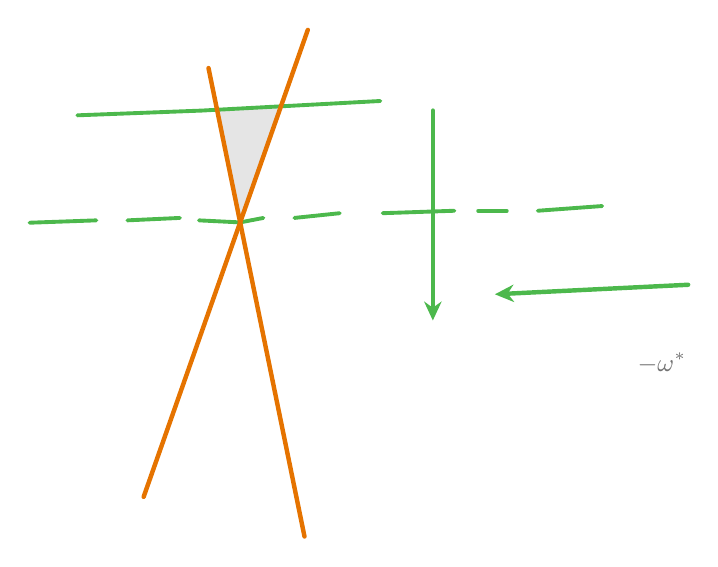
\begin{tikzpicture}[x=1mm,y=1mm,line cap=round,line join=round,font=\scriptsize]
\fill[black!10] (30.38,-27.84) -- (27.45,-13.53) -- (35.56,-13.1) -- cycle;
\draw[Lg,line width=1.4pt] (9.7,-14.24) -- (25.45,-13.64) -- (48.18,-12.42);
\draw[Lg,line width=1.4pt] (3.64,-27.88) -- (12.12,-27.58);
\draw[Lg,line width=1.4pt] (16.06,-27.58) -- (22.73,-27.27);
\draw[Lg,line width=1.4pt] (25.15,-27.58) -- (30.38,-27.84) -- (33.33,-27.27);
\draw[Lg,line width=1.4pt] (37.27,-27.27) -- (43.03,-26.67);
\draw[Lg,line width=1.4pt] (48.48,-26.67) -- (57.58,-26.36);
\draw[Lg,line width=1.4pt] (60.61,-26.36) -- (64.24,-26.36);
\draw[Lg,line width=1.4pt] (68.18,-26.36) -- (76.36,-25.76);
\draw[Or,line width=1.6pt] (26.36,-8.24) -- (30.38,-27.84) -- (38.55,-67.73);
\draw[Or,line width=1.6pt] (38.97,-3.39) -- (30.38,-27.84) -- (18.12,-62.7);
\draw[Lg,line width=1.6pt,-{Stealth[length=2.4mm,width=2.2mm]}] (54.85,-13.64) -- (54.85,-40.3);
\draw[Lg,line width=1.6pt,-{Stealth[length=2.4mm,width=2.2mm]}] (87.27,-35.76) -- (62.73,-36.97);
\node[pencil,inner sep=1pt] at (83.94,-45.76) {\small $-\omega^{*}$};
\end{tikzpicture}
\end{document}
